\section{プロトタイプ検出器のデザイン}
\subsection{}
\subsection{コーン型ライトガイドの深さ最適化}
今回のテスト実験では、セグメントサイズの違いによる分解能への影響を理解するために図\ref{fig:cone}の様な
2種類のコーン型ライトガイドを製作した。\\
先行研究からセグメントサイズは50 mm以下が要求されているので、入口直径は50 mmとより小さい30 mmとした。
MPPCを取り付けるため、出口直径はどちらもMPPCの対角線の長さとなる8.5 mmとした。
ここで、各コーンの深さによって集光効率が変わるため、最適な深さをGEANT4によるシミュレーションを用いて決定した。
まず、図の様にコーン入口に対して垂直に光子を入射させ、コーンの深さを変えながら式で定義される収率をもとに最適な深さを決定した。
図から、50 mmコーンは110 mm, 30 mmコーンは31 mm以上の深さが良いことが分かった。
今回は、設計に余裕を持たせるため50 mmコーンは深さ120 mm,30 mmコーンは深さ33 mmのものを製作した。
\begin{figure}[htbp]
  \centering
  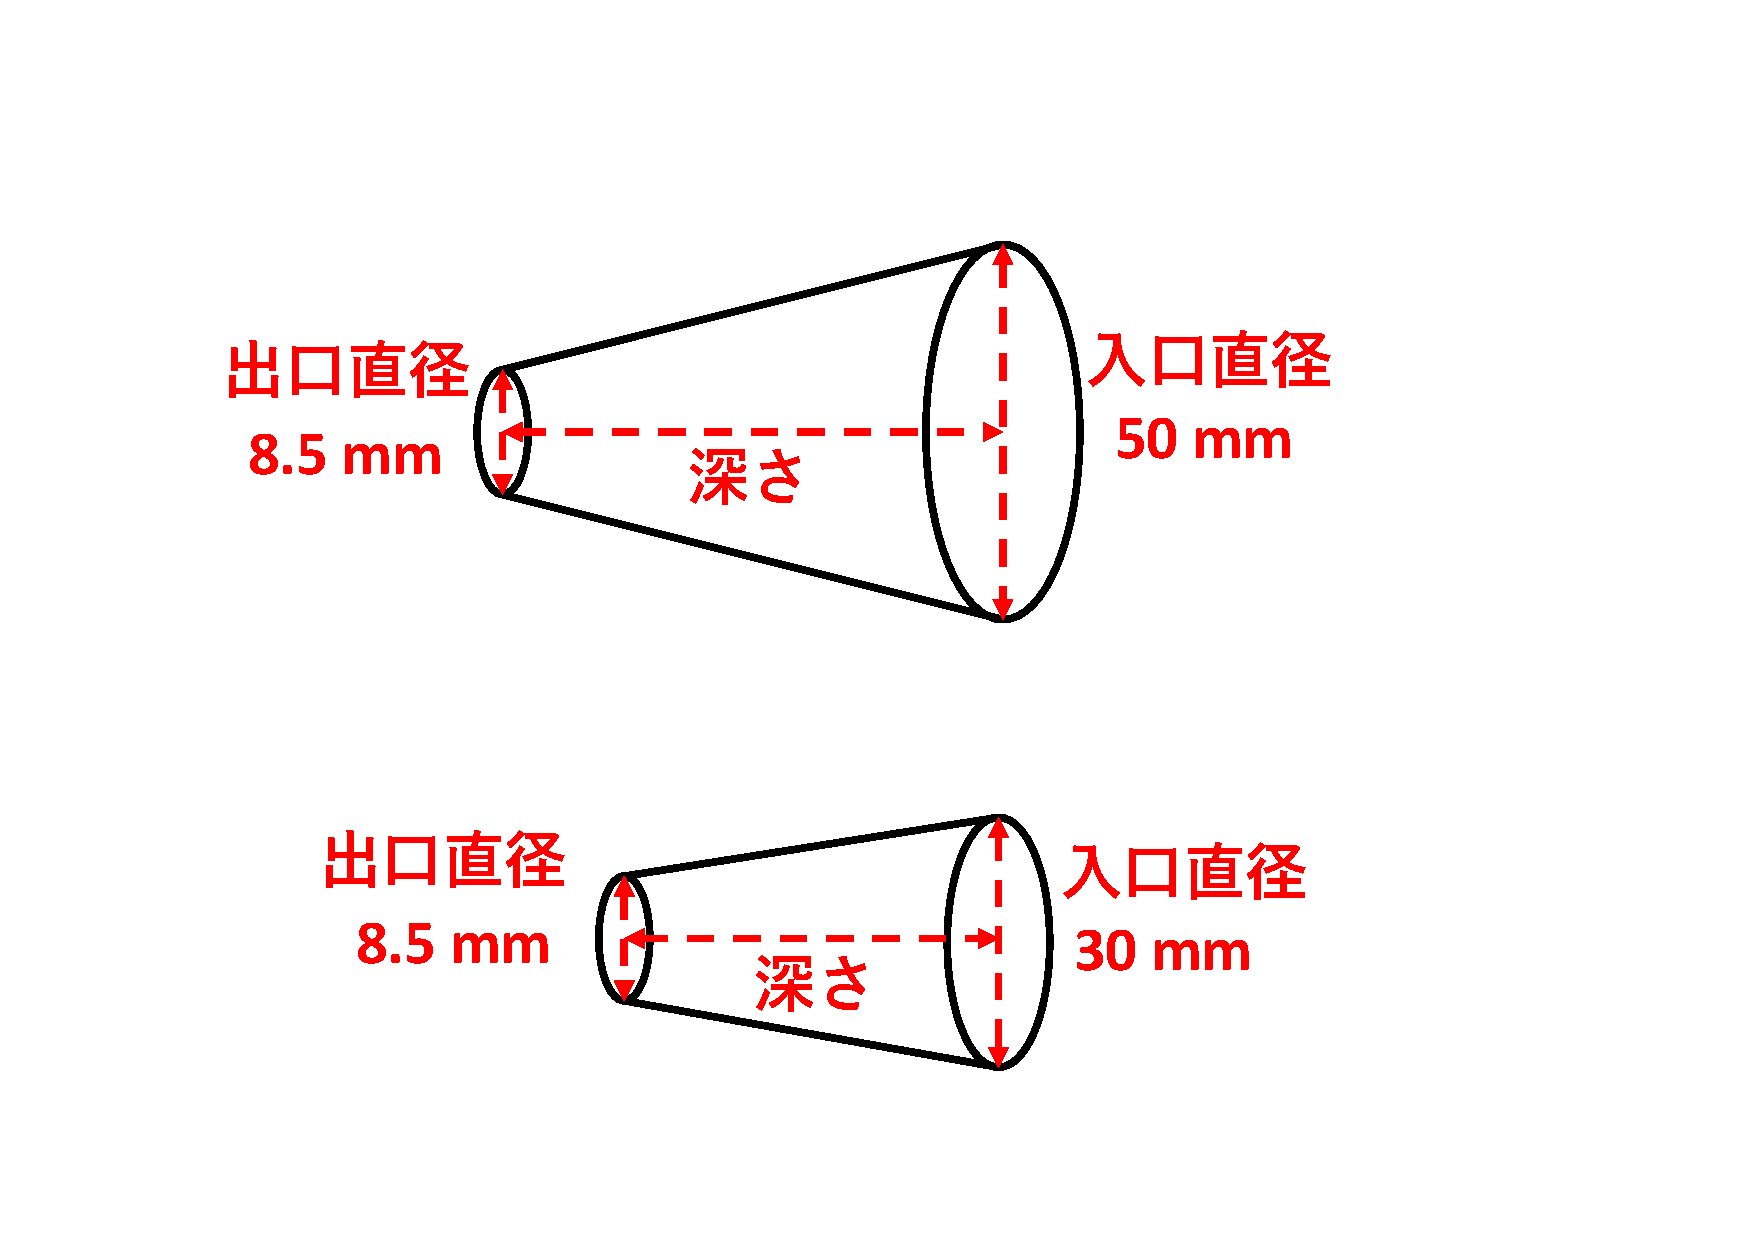
\includegraphics[width=10cm]{images/chapter3/cone.pdf}
  \caption{コーン型ライトガイドの模式図。入口直径が50 mmの場合と30 mmの場合。}
  \label{fig:cone}
\end{figure}

\subsection{検出面の配置}